\section{Background Material}

We begin with a review of the material necessary to understand standard persistent homology. We use $\mathbf{N}$, $\mathbf{Z}$ and $\mathbf{R}$ to denote the natural numbers, integers and real numbers respectively, as we reserve blackboard bold to later denote persistence modules.

\subsection{Free modules}

\begin{definition}
A \emph{module over a ring $R$}, or \emph{$R$-module}, is an abelian group $M$ equipped with an action of $R$ satisfying the following properties. Let $1_R$ denote the multiplicative identity of the ring, and $rx$ the action of the ring element $r$ on the module element $x$. For any $r, s \in R$ and $x, y \in M$:
\begin{itemize}
\itemsep0em
\item $r(x + y) = rx + ry$;
\item $(r + s)x = rx + sx$;
\item $(rs)x = r(sx)$;
\item $1_R x = x$.
\end{itemize}
\end{definition}

\begin{example}
If we take $R$ to be a field, the above conditions are the conditions of a vector space, thus, a vector space over $F$ is precisely an $F$-module.
\end{example}

\begin{example}
Any abelian group $M$ is a $\mathbf{Z}$-module via the action $nx = \underbrace{x + \dots + x}_{n \text{ times}}$. Abelian groups are often referred to as $\mathbf{Z}$-modules for this reason.
\end{example}

\begin{definition}
The \emph{free $R$-module on a set $S$} is the module formed by taking every formal linear combination of elements of $S$ with coefficients in $R$. These linear combinations are given an $R$-module structure as follows. Let $a_i, b_i \in R$ and $s_i \in S$, then:
\begin{align*}
(a_1 s_1 + a_2 s_2 + \dots) + (b_1 s_1 + b_2 s_2 + \dots) &= (a_1 + b_1) s_1 + (a_2 + b_2) s_2 + \dots; \\
a (a_1 s_1 + a_2 s_2 + \dots) &= (a a_1) s_1 + (a a_2) s_2 + \dots
\end{align*}

The \emph{free abelian group on $S$} is the free $\mathbf{Z}$-module on $S$.
\end{definition}

\subsection{Graded rings and modules}

\begin{definition}
A \emph{graded ring} is a ring with a decomposition into abelian groups:
\begin{align*}
  R = \bigoplus_{n \in \mathbf{N}} R_n
\end{align*}
such that multiplication satisfies $R_n R_m \subseteq R_{n+m}$. Elements of any $R_n$ are called \emph{homogeneous elements of degree $n$} and for any $r \in R_n$ we write $\deg r = n$.
\end{definition}

\begin{example}
The prototypical example of a graded ring is the polynomial ring $R[t]$, which decomposes as:
\begin{align*}
  R[t] = \bigoplus_{n \in \mathbf{N}} t^n \cdot R.
\end{align*}
\end{example}

Given a module over a graded ring, we can have the module structure respect the grading of the ring.

\begin{definition}
A \emph{graded module} over a graded ring $R$ is a module $M$ with a decomposition:
\begin{align*}
  M = \bigoplus_{n \in \mathbf{N}} M_n
\end{align*}
where the action of $R$ satisfies $R_n M_m \subseteq M_{n+m}$.
\end{definition}

We will see that the structure of standard persistent homology is equivalent to a graded module over a particular ring.

\subsection{Structure theorem}

Recall that a \emph{principal ideal domain} (PID) is an integral domain in which every ideal is generated by one element. Such ideals are called \emph{principal} ideals.

\begin{example}
The integers $\mathbf{Z}$ are a simple example of a PID. Given any ideal, we can find the greatest common divisor of all its elements. This element must generate the whole ideal.

For an example of a ring that is \emph{not} a PID, consider the ring $\mathbf{Z}[x]$. The ideal $\langle x, 2 \rangle$ cannot be generated by one element.
\end{example}

\begin{example}
For our purposes, an important example of a PID is the polynomial ring $\k[x]$, where $\k$ is a field.
\end{example}

Finitely generated modules over a PID can be uniquely decomposed using a generalisation of the structure theorem for finitely generated abelian groups \cite{dummit-foote}.

\begin{theorem}
If $R$ is a PID, every finitely generated module over $R$ is isomorphic to one of the form
\begin{align*}
R^\beta \oplus \left( \bigoplus_{i=1}^m R / \langle d_i \rangle \right)
\end{align*}
where $d_i \in R$, $\beta \in \mathbf{N}$, and $d_i \mid d_{i+1}$.
\end{theorem}

When $R = \mathbf{Z}$, we recover the structure theorem for finitely generated abelian groups. Given a graded module, we can say more:

\begin{theorem}
\label{thm:graded-pid-structure}
Every graded module over a PID $R$ is isomorphic to one of the form
\begin{align*}
\left( \bigoplus_{i=1}^n \Sigma^{\alpha_i} R \right) \oplus \left( \bigoplus_{i=1}^m \Sigma^{\gamma_i} R / \langle d_i \rangle \right)
\end{align*}
where $d_i \in R$ are homogeneous elements with $d_i | d_{i+1}$, $\alpha_i, \gamma_j \in \N$. The symbol $\Sigma^k$ denotes a formal upward shift of $k$ steps in the grading, i.e., $\Sigma^k R$ is the graded ring with $(\Sigma^k R)_n = R_{n - k}$.
\end{theorem}

\subsection{Simplicial complexes}
To begin with, we restrict our focus to a class of topological spaces that have a particularly simple description: simplicial complexes. Intuitively, these are spaces constructed of vertices, edges, triangles, tetrahedra, and so on, with these shapes glued together along their `faces'.

\begin{definition}
An \emph{abstract simplicial complex} $K = (V, S)$ is a set $V$ together with a collection $S$ of subsets of $V$ called \emph{simplices} such that for every $v \in V$, $\{v\} \in S$, and if $\tau \subseteq \sigma \in S$, then also $\tau \in S$.

The subsets $\{v\}$ of $V$ are called the \emph{vertices} of $K$. A simplex $\sigma \in S$ is of dimension $k$ if $\sigma$ has $k+1$ elements. If $\tau \subset \sigma$, we say $\tau$ is a \emph{face} of $\sigma$.

An \emph{oriented} simplex is a simplex together with a choice of orientation for that simplex. Any ordering of the vertices determines an orientation, and two orientations are considered equivalent if they differ by an even permutation. We write $[\omega]$ for an oriented simplex, and use the ordered sequence $[v_1, v_2, \dots]$ to denote the oriented simplex with vertices $\{v_1, v_2, \dots \}$ and the given orientation.
\end{definition}

\begin{example}
We will use the following simplicial complex as a running example. Let $K = (V, S)$ with:
\begin{align*}
  V &= \{a, b, c, d\} \\
  S &= \{\emptyset, \{a\}, \{b\}, \{c\}, \{d\}, \{a, b\}, \{a, c\}, \{a, d\}, \{b, d\}, \{d, c\}, \{a, b, d\}\}
\end{align*}
\end{example}

Abstract simplicial complexes are useful in practice because of their simple structure and combinatorial properties. In theoretical settings, it is more convenient to consider general topological spaces.

We can associate a topological space to an abstract simplicial complex by pairing each $k$-dimensional subset in $S$ with the convex hull of $k+1$ independent points in $\mathbf{R}^d$ for some $d \geq k$. Such a space is called a \emph{geometric realisation}. With this pairing we recover the notions of shape we are familiar with: 1-simplices correspond to edges, 2-simplices to triangles and so on. In such a realisation we require that the nontrivial intersection of any two simplices is one of their common faces.

\begin{figure}[h]
\centering
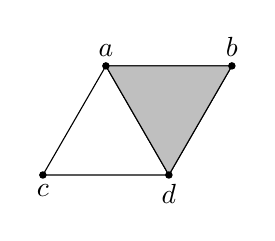
\begin{tikzpicture}[scale=0.4]
  \coordinate[label=above:$a$] (a) at (2,3.464);
  \coordinate[label=above:$b$] (b) at (6,3.464);
  \coordinate[label=below:$c$] (c) at (0,0);
  \coordinate[label=below:$d$] (d) at (4,0);

  \draw (a) -- (d) -- (c) -- cycle;
  \draw (d) -- (b) -- (a);
  \draw[fill=gray!50] (a) -- (d) -- (b) -- cycle;
  \draw[black,fill] (a) circle [radius=0.1cm] ;
  \draw[black,fill] (b) circle [radius=0.1cm] ;
  \draw[black,fill] (c) circle [radius=0.1cm] ;
  \draw[black,fill] (d) circle [radius=0.1cm] ;
\end{tikzpicture}
\caption{The simplicial complex $K$}
\label{fig:simplicial}
\end{figure}

\begin{example}
Figure~\ref{fig:simplicial} shows one realisation of our abstract simplicial complex $K$.
\end{example}

Given any abstract simplicial complex $K$, we can always construct a geometric realisation.

\begin{theorem}
Every abstract simplicial complex has a geometric realisation.
\end{theorem}
\begin{proof}
Let $n$ be the number of vertices in the simplicial complex $K$. Choose a one-to-one correspondence between the vertices of $K$ and the unit vectors $\{e_1, e_2, \dots, e_n\}$ in $\mathbf{R}^n$. For each simplex in $K$, construct the convex hull of the corresponding points in $\mathbf{R}^n$. By construction, these convex hulls intersect either on a common face or not at all. Our geometric realisation is the union of these convex hulls, inheriting the subspace topology of $\mathbf{R}^n$.
\end{proof}

We will refer to an abstract simplicial complex and its realisation interchangeably.

\subsection{Simplicial homology}

Homology is a procedure that, given a topological space, produces a sequence of abelian groups, $H_k$, that represent the `holes' in the space. This set of groups is a topological invariant; any two homeomorphic spaces have the same homology groups. There are a number of different types of homology. We begin by introducing simplicial homology, which can only be applied to simplicial complexes.

The $k$-th homology group, $H_k(K)$, describes the $k$-dimensional holes in $K$. For example, the `hole' in the middle of a circle is a 1-dimensional hole, so $H_1(\mathbb{S}^1)$ has rank 1. A 0-dimensional hole is interpreted as a gap between two components, so $H_0$ counts the path-connected components of $K$.

\begin{example}
Consider the $n$-sphere $\mathbb{S}^n$. The homology groups are as follows:
\begin{align*}
  H_k(\mathbb{S}^n) = \begin{cases}
    \mathbf{Z} & k = 0 \text{ or } n ;\\
    0 & \text{otherwise.}
\end{cases}
\end{align*}
The non-trivial $H_0$ represents the single connected component of $\mathbb{S}^n$, and non-trivial $H_n$ the $n$-dimensional hole.
\end{example}

\begin{example}
Consider the standard embedding of a torus $\mathbb{T}$ in $\R^3$. The torus has a single component, two 1-dimensional holes (one circle through the middle, one running around the loop), and one 2-dimensional hole (the void inside the torus). The corresponding homology groups are:
\begin{align*}
  H_k(\mathbb{T}) = \begin{cases}
    \mathbf{Z} & k = 0 \\
    \mathbf{Z} \oplus \mathbf{Z} & k = 1 \\
    \mathbf{Z} & k = 2 \\
    0 & \text{otherwise.}
\end{cases}
\end{align*}
\end{example}

\begin{definition}
The \emph{$k$-th chain group} of $K$, denoted $C_k$, is the free abelian group with basis the set of oriented simplices of $K$, where we let $[\sigma] = -[\tau]$ if $\sigma$ and $\tau$ are the same simplex with the opposite orientation.
\end{definition}

Elements of $C_k$ are known as $k$-chains, and have the form $c = \sum_i n_i [\sigma_i]$, with $\sigma_i$ $k$-simplices in $K$.

Let $\sigma$ be a $k$-simplex with vertices $[v_0, \cdots, v_k]$. Given such a $k$-simplex, we would like to calculate its boundary, $\del_k \sigma$. The faces of $\sigma$ are the $(k-1)$-simplices with vertex sets of the form $[v_0, \cdots, \hat{v_i}, \cdots, v_k]$, where $\hat{v_i}$ indicates that $v_i$ is deleted from the sequence. We might expect the boundary to be the chain given by the sum of the faces, but a better choice is the following
\begin{align*}
\del_k[\sigma] = \del_k[v_0, \cdots, v_k] = \sum_i (-1)^i [v_0, \cdots, \hat{v_i}, \cdots, v_k].
\end{align*}
When the dimension is unambiguous, we write $\del$ for $\del_k$.

\begin{example}
For generic simplices of dimension 0,1,2:
\begin{align*}
  &\del[v_0] = 0 \\
  &\del[v_0, v_1] = [v_1] - [v_0] \\
  &\del[v_0, v_1, v_2] = [v_1, v_2] - [v_0, v_2] + [v_0, v_1]
\end{align*}
\end{example}

Intuitively, we make this definition so that orientations are kept consistent as we travel around the boundary of a simplex.

The boundary operator $\del_k$ can be turned into a homomorphism $C_k \to C_{k-1}$ by extending it linearly on the basis elements of $C_k$. Together, these groups and maps form what is known as a \emph{chain complex}, $C_*$.
\begin{displaymath}
\xymatrix{
\cdots \ar[r] & C_{k+1} \ar[r]^{\del_{k+1}} & C_{k} \ar[r]^{\del_k} & C_{k-1} \ar[r] & \cdots
}
\end{displaymath}

The boundary operator allows us to define two important subgroups of each $C_k$: the \emph{cycle group} $Z_k = \ker \del_k$ and the \emph{boundary group} $B_k = \im \del_{k+1}$. These groups match with our intuition of what a cycle and boundary should be; a cycle generalises a closed loop or surface, and a boundary is a cycle that bounds a higher dimensional shape.

\begin{figure}[h]
\centering
\begin{tikzpicture}[scale=0.4]
  \coordinate[label=above:$a$] (a) at (2,3.464);
  \coordinate[label=above:$b$] (b) at (6,3.464);
  \coordinate[label=below:$c$] (c) at (0,0);
  \coordinate[label=below:$d$] (d) at (4,0);

  \draw[fill=gray!50] (a) -- (d) -- (b) -- cycle;
  \begin{scope}[very thick,decoration={
      markings,
      mark=at position 0.5 with {\arrow{>}}}
      ]
      \draw[postaction={decorate}] (a) -- (b);
      \draw[postaction={decorate}] (b) -- (d);
      \draw[postaction={decorate}] (d) -- (c);
      \draw[postaction={decorate}] (c) -- (a);
  \end{scope}

  \draw (a) -- (d);
  \draw[black,fill] (a) circle [radius=0.1cm] ;
  \draw[black,fill] (b) circle [radius=0.1cm] ;
  \draw[black,fill] (c) circle [radius=0.1cm] ;
  \draw[black,fill] (d) circle [radius=0.1cm] ;
\end{tikzpicture}
\caption{$K$ with the cycle $[a, b] + [b, d] - [c, d] - [a, c]$ highlighted}
\label{fig:cycle}
\end{figure}

\begin{figure}[h]
\centering
\begin{tikzpicture}[scale=0.4]
  \coordinate[label=above:$a$] (a) at (2,3.464);
  \coordinate[label=above:$b$] (b) at (6,3.464);
  \coordinate[label=below:$c$] (c) at (0,0);
  \coordinate[label=below:$d$] (d) at (4,0);

  \draw[fill=gray!50] (a) -- (d) -- (b) -- cycle;
  \begin{scope}[very thick,decoration={
      markings,
      mark=at position 0.5 with {\arrow{>}}}
      ]
      \draw[postaction={decorate}] (a) -- (b);
      \draw[postaction={decorate}] (b) -- (d);
      \draw[postaction={decorate}] (d) -- (a);
  \end{scope}

  \draw (a) -- (c) -- (d);
  \draw[black,fill] (a) circle [radius=0.1cm] ;
  \draw[black,fill] (b) circle [radius=0.1cm] ;
  \draw[black,fill] (c) circle [radius=0.1cm] ;
  \draw[black,fill] (d) circle [radius=0.1cm] ;
\end{tikzpicture}
\caption{$K$ with the boundary $\del [a, b, d]$ highlighted}
\label{fig:boundary}
\end{figure}

\begin{example}
Returning to our earlier example, the chain $[a, b] + [b, d] - [c, d] - [a, c]$ is an element of $Z_1$, as:
\begin{align*}
  \del([a, b] + [b, d] - [c, d] - [a, c]) &= \del[a, b] + \del[b, d] - \del[c, d] - \del[a, c] \\
  &= ([b] - [a]) + ([d] - [b]) - ([d] - [c]) - ([c] - [a]) \\
  &= 0
\end{align*}
We represent an oriented simplex $[x, y]$ as an arrow pointing $x \to y$. This chain is shown in Figure~\ref{fig:cycle}.

The chain $\del [a,b,d] = [b, d] - [a, d] + [a, b]$ is an element of $B_1$. This chain is shown in Figure~\ref{fig:boundary}. In fact, this chain is a generator for the group $B_1$, as $[a,b,d]$ is the only 2-simplex. Note the consistent orientation of the edges.
\end{example}

\begin{proposition}
For any $k$, $\del_{k-1} \circ \del_k = 0$.
\end{proposition}
\begin{proof}
By definition,
\begin{align*}
\del_k[v_0, \cdots, v_k] = \sum_i (-1)^i [v_0, \cdots, \hat{v_i}, \cdots, v_k]
\end{align*}
Then,
\begin{align*}
\del_{k-1}\del_k[v_0, \cdots, v_k] &= \sum_{j<i} (-1)^i (-1)^j [v_0, \cdots, \hat{v_j}, \cdots, \hat{v_i}, \cdots, v_k] \\
& \quad + \sum_{j>i} (-1)^i (-1)^{j-1} [v_0, \cdots, \hat{v_i}, \cdots, \hat{v_j}, \cdots, v_k] \\
&= \sum_{j<i} (-1)^i (-1)^j [v_0, \cdots, \hat{v_j}, \cdots, \hat{v_i}, \cdots, v_k] \\
& \quad - \sum_{j<i} (-1)^i (-1)^j [v_0, \cdots, \hat{v_j}, \cdots, \hat{v_i}, \cdots, v_k] \\
&= 0
\end{align*}
where in the second sum we swap the roles of $i$ and $j$.
\end{proof}

This Proposition implies the inclusion $B_k \subseteq Z_k$.

\begin{definition}
The \emph{$k$-th simplicial homology group} of $K$ is $H_k = Z_k / B_k$. Elements of $H_k$ are equivalence classes of `homologous' cycles.
\end{definition}

\begin{example}
Let us calculate $H_1$ of our complex $K$. This is easiest when we choose compatible bases for $Z_1$ and $B_1$. Let $\sigma$ and $\tau$ be the cycles:
\begin{align*}
  \sigma &= [a, b] + [b, d] - [a, d] \\
  \tau &= [a, d] - [c, d] - [a, c]
\end{align*}
It is not too hard to see that the cycle and boundary groups are
\begin{align*}
  Z_1 &= \langle \sigma, \tau \rangle \\
  B_1 &= \langle \sigma \rangle \\
\intertext{and therefore,}
  H_1 &= Z_1 / B_1 = \langle \tau \rangle \cong \mathbf{Z}.
\end{align*}

This is the answer we expect, as our simplicial complex $K$ has one 1-dimensional hole by inspection.
\end{example}

\begin{definition}
The \emph{$k$-th Betti number} of $K$, $\beta_k$, is the rank of the free submodule of $H_k$.
\end{definition}

\subsection{Singular homology}

We would like to define a notion of homology that applies to all topological spaces, not just simplicial complexes. Rather than considering spaces constructed from simplices, we will consider arbitrary continuous maps from simplices into our space.

\begin{definition}
The \emph{standard $k$-simplex $\Delta^k$} is the convex hull of the standard unit vectors $\{e_1, e_2, \dots e_{k+1}\}$ in $\mathbf{R}^{k+1}$.
\end{definition}

\begin{definition}
A \emph{singular $k$-simplex} in a topological space $X$ is a continuous map $\sigma : \Delta^k \to X$.
\end{definition}

The image of $\sigma$ may not resemble a simplex at all; all that is required is that $\sigma$ be continuous. Now let $C_k$ be the free abelian group with basis the set of singular $k$-simplices in $X$. As before, elements of $C_k$ are called (singular) $k$-chains and have the form $c = \sum_i n_i \sigma_i$.

We define our boundary map $C_{k+1} \to C_k$ using a formula analogous to that in simplicial homology:
\begin{align*}
\del_k(\sigma) = \sum_i (-1)^i \sigma |_{[v_0, \cdots, \hat{v_i}, \cdots, v_k]}.
\end{align*}
Here we implicitly identify $[v_0, \cdots, \hat{v_i}, \cdots, v_k]$ with $\Delta^{k-1}$, so $\sigma |_{[v_0, \cdots, \hat{v_i}, \cdots, v_k]}$ becomes a map $\Delta^{k-1} \to X$, i.e., a singular $(k-1)$-simplex.

\begin{definition}
The \emph{$k$th singular homology group} of $K$ is $H_k = Z_k / B_k = \ker \del_k / \im \del_{k+1}$.
\end{definition}

Because each $C_k$ is so tremendously large, it is not clear that $H_k$ defined in this way gives a useful invariant. However, in the case of simplicial complexes we have the following theorem.

\begin{theorem}
The simplicial homology of a simplicial complex is isomorphic to the singular homology of its geometric realisation.
\end{theorem}
\begin{proof}
See Hatcher \cite{hatcher}.
\end{proof}

Given a continuous map between topological spaces, there should be some relationship between the homology groups.

\begin{theorem}
A continuous map $f : X \to Y$ induces a homomorphism $f_* : H_k(X) \to H_k(Y)$ for all $k$.
\end{theorem}
\begin{proof}
The map $f : X \to Y$ induces a map $f_\# : C_k(X) \to C_k(Y)$ as follows. Given any $k$-simplex $\sigma : \Delta^k \to X$, we can compose with $f$ to get a $k$-simplex $f_\#(\sigma) = f \sigma : \Delta^k \to Y$. Extending this map linearly via $f_\#(\sum_i n_i \sigma_i) = \sum_i n_i f_\#(\sigma_i)$ gives us the required map $C_k(X) \to C_k(Y)$.

This map $f_\#$ satisfies $f_\# \del = \del f_\#$, as:
\begin{align*}
  f_\#\del(\sigma) &= f_\#(\sum_i (-1)^i \sigma |_{[v_0, \cdots, \hat{v_i}, \cdots, v_k]}) \\
  &= \sum_i (-1)^i f \sigma |_{[v_0, \cdots, \hat{v_i}, \cdots, v_k]} = \del f_\#(\sigma).
\end{align*}

We have that $f_\#$ sends boundaries to boundaries as $\del f_\#(\sigma) = f_\# \del(\sigma)$. It also sends cycles to cycles, as $\del \sigma = 0$ implies $\del f_\#(\sigma) = f_\# \del(\sigma) = 0$.

Therefore $f_\#$ induces a homomorphism $f_* : H_k(X) \to H_k(Y)$.
\label{homology-functor}
\end{proof}

Earlier, when we defined the chain groups using free abelian groups, we implicitly chose our \emph{ground ring} $R$ to be the integers. We can generalise this to any ring $R$ by defining the chain groups to be free $R$-modules. Our homology groups $H_k$ then also become $R$-modules, and we write $H_k(X ; R)$ for homology with coefficients in $R$. When $R$ is a field, the torsion disappears and the homology group $H_k$ is a vector space. The homology group is completely described by the integer $\beta_k$, which may depend on the chosen field.

\subsection{Filtrations}

In its most general sense, a filtration of some mathematical structure $S$ is a collection of subsets $\{S_i\}$ with index set $I$, such that $i \leq j \in I$ implies $S_i \subseteq S_j$. For persistent homology we are interested in filtrations of topological spaces. 

\begin{definition}
Given a subset $A \subset \mathbf{R}$, a \emph{filtration} of a topological space $X$ is a family of subspaces $\{X_\alpha\}_{\alpha \in A}$ that are nested with respect to inclusion, that is, for all $\alpha \leq \alpha'$, $X_\alpha \subseteq X_{\alpha'}$. We use $X^*$ to denote a filtration of $X$.
\end{definition}

An important type of filtration is one formed by sublevel sets of a real-valued function on a space. Given a function $f : X \to \mathbf{R}$, let $X_a = f^{-1}((-\infty, a])$ be the sublevel set. It is clear that for $a \leq b$, $X_a \subseteq X_b$. This gives us a filtration $X^f = \{ X_a \}_{a \in \mathbf{R}}$.

For simplicial complexes, it is more natural to consider filtrations where each intermediate space is also a simplicial complex.

\begin{definition}
A \emph{filtration} of a simplicial complex $K = (V, S)$ is a function $\rho : S \to \mathbf{R}$, such that for any face $\tau \subseteq \sigma$, $\rho(\tau) \leq \rho(\sigma)$. This monotonicity guarantees that for all $a \in \mathbf{R}$, $K_a = \rho^{-1}((-\infty, a])$ is a valid simplicial complex. Let $\{\rho_i\}_{i = 1 \dots n}$ be the values $\rho$ takes on the simplices of $K$. We then have the following sequence of subcomplexes:
\begin{align*}
\emptyset = K_0 \subseteq K_1 \subseteq \dots \subseteq K_n = K
\end{align*}
\end{definition}

\begin{figure}
\makebox[\linewidth]{
\renewcommand{\arraystretch}{1.5}
\begin{tabular}{| c | c | c | c | c |}
\hline
\begin{tikzpicture}[scale=0.4]
\end{tikzpicture} &
\begin{tikzpicture}[scale=0.4]
  \coordinate[label=above:$a$] (a) at (2,3.464);
  \coordinate[label=above:$b$] (b) at (6,3.464);
  \coordinate[label=below:] (c) at (0,0);
  \coordinate[label=below:] (d) at (4,0);

  \draw[black,fill] (a) circle [radius=0.1cm] ;
  \draw[black,fill] (b) circle [radius=0.1cm] ;
\end{tikzpicture} &
\begin{tikzpicture}[scale=0.4]
  \coordinate[label=above:$a$] (a) at (2,3.464);
  \coordinate[label=above:$b$] (b) at (6,3.464);
  \coordinate[label=below:$c$] (c) at (0,0);
  \coordinate[label=below:$d$] (d) at (4,0);

  \draw (a) -- (b) -- (d);
  \draw[black,fill] (a) circle [radius=0.1cm] ;
  \draw[black,fill] (b) circle [radius=0.1cm] ;
  \draw[black,fill] (c) circle [radius=0.1cm] ;
  \draw[black,fill] (d) circle [radius=0.1cm] ;
\end{tikzpicture} &
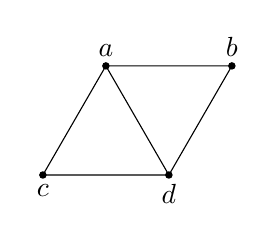
\begin{tikzpicture}[scale=0.4]
  \coordinate[label=above:$a$] (a) at (2,3.464);
  \coordinate[label=above:$b$] (b) at (6,3.464);
  \coordinate[label=below:$c$] (c) at (0,0);
  \coordinate[label=below:$d$] (d) at (4,0);

  \draw (a) -- (d) -- (c) -- cycle;
  \draw (d) -- (b) -- (a);
  \draw[black,fill] (a) circle [radius=0.1cm] ;
  \draw[black,fill] (b) circle [radius=0.1cm] ;
  \draw[black,fill] (c) circle [radius=0.1cm] ;
  \draw[black,fill] (d) circle [radius=0.1cm] ;
\end{tikzpicture} &
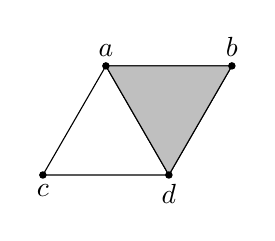
\begin{tikzpicture}[scale=0.4]
  \coordinate[label=above:$a$] (a) at (2,3.464);
  \coordinate[label=above:$b$] (b) at (6,3.464);
  \coordinate[label=below:$c$] (c) at (0,0);
  \coordinate[label=below:$d$] (d) at (4,0);

  \draw (a) -- (d) -- (c) -- cycle;
  \draw (d) -- (b) -- (a);
  \draw[fill=gray!50] (a) -- (d) -- (b) -- cycle;
  \draw[black,fill] (a) circle [radius=0.1cm] ;
  \draw[black,fill] (b) circle [radius=0.1cm] ;
  \draw[black,fill] (c) circle [radius=0.1cm] ;
  \draw[black,fill] (d) circle [radius=0.1cm] ;
\end{tikzpicture} \\
\hline
$\emptyset = K_0$ & $K_1$ & $K_2$ & $K_3$ & $K_4 = K$ \\
\hline
\end{tabular}
}
\caption{A filtration of $K$}
\label{fig:filtration}
\end{figure}

\begin{example}
Figure~\ref{fig:filtration} shows one possible filtration of our space $K$.
\end{example}

A practical source of filtered complexes comes from point cloud data.

\begin{definition}
Let $(X, d_X)$ be a metric space. The \emph{Vietoris-Rips complex of $X$} with parameter $\alpha$ is the simplicial complex with vertex set $X$ and simplices given by subsets of $X$ that are mutually no more than $\alpha$ distance apart. In other words,
\begin{align*}
  \mathbf{VR}(X, \alpha) = \{ \sigma \subseteq X \st d_X(x_i, x_j) \leq \alpha \text{ for all } x_i, x_j \in \sigma \}.
\end{align*}
\end{definition}


\begin{figure}
\makebox[\linewidth]{
\newcommand{\vrcomplex}[2][0.5]{
\begin{center}
\begin{tikzpicture}[scale=#1]
  \coordinate (a) at (2,3.3);
  \coordinate (b) at (7,4);
  \coordinate (c) at (0,0);
  \coordinate (d) at (3.5,0);

\clip (-3, -3) rectangle (10, 7);
\draw[white, fill, opacity=0] (-3, -3) rectangle (10, 7);

  \draw[black,fill] (a) circle [radius=0.1cm];
  \draw[black,fill] (b) circle [radius=0.1cm];
  \draw[black,fill] (c) circle [radius=0.1cm];
  \draw[black,fill] (d) circle [radius=0.1cm];

\draw[cyan, fill, opacity= 0.3] (a) circle (#2cm);
\draw[black] (a) circle (#2cm);
\draw[cyan, fill, opacity= 0.3] (b) circle (#2cm);
\draw[black] (b) circle (#2cm);
\draw[cyan, fill, opacity= 0.3] (c) circle (#2cm);
\draw[black] (c) circle (#2cm);
\draw[cyan, fill, opacity= 0.3] (d) circle (#2cm);
\draw[black] (d) circle (#2cm);
\end{tikzpicture}
\end{center}
}

\newcommand{\annuluscomplex}[1]{
\begin{figure}
\noindent\makebox[\textwidth]{%
\begin{tikzpicture}[scale=0.3]
%\begin{tikzpicture}[remember picture, overlay, scale=0.3]
%\tikzset{shift={(current page.center)},yshift=0cm}
\clip (-20, -10) rectangle (20, 10);
\draw[white, fill, opacity=0] (-20, -10) rectangle (20, 10);

\def\points{8.092593/0.134148,8.447231/0.949326,7.658496/1.144397,8.815373/2.177150,8.398666/2.076670,
9.006517/3.977381,7.520945/2.129330,6.698849/2.255754,5.807683/2.718666,7.062904/3.015901,
7.278569/4.457003,5.898714/4.987420,4.562342/5.118081,4.727490/6.667248,4.005391/6.592861,
3.983471/7.332549,4.038059/8.096364,3.859597/8.469849,3.195593/6.353141,3.981205/6.389805,
2.429519/8.228017,3.216939/6.555953,1.802313/7.954675,2.259787/8.041740,-0.397224/9.074358,
0.401439/7.953553,-1.266806/7.655207,-0.623094/8.432865,-1.053032/8.554193,-3.427812/7.770895,
-3.352173/7.103145,-3.918641/6.328826,-3.049035/7.426226,-2.966824/6.214639,-4.897973/5.293921,
-4.003319/7.130895,-4.712890/5.274353,-7.091653/5.528760,-5.655604/5.897540,-6.628111/4.522957,
-5.341439/5.245499,-8.360414/3.793542,-7.223336/4.216060,-7.555821/3.819587,-7.634792/2.563077,
-6.865465/0.812593,-8.336023/1.255058,-7.045293/1.036940,-8.049704/0.071260,-9.388684/-0.655015,
-8.968349/0.711340,-7.298501/-0.970684,-7.979053/-0.100698,-8.845275/-2.088935,-8.152570/-1.446517,
-7.195373/-3.045787,-8.253632/-2.281902,-6.395403/-2.900581,-7.635319/-4.477232,-5.337140/-5.388422,
-6.981240/-4.074050,-5.165616/-3.986240,-6.545813/-6.218857,-5.876391/-5.532203,-6.071537/-6.550160,
-4.202732/-5.660057,-3.449910/-6.121640,-3.412754/-8.166190,-3.313574/-6.292893,-2.183215/-6.090390,
-1.688938/-7.667467,-1.101403/-6.677577,-0.731159/-7.654493,0.701523/-9.010581,-1.000123/-8.899405,
1.008500/-8.270074,0.095397/-7.204591,0.247374/-6.901711,2.207983/-6.904603,2.225776/-8.183645,
2.731266/-7.370991,3.809154/-8.507204,4.589025/-8.216510,3.768458/-7.888926,5.126484/-5.980651,
4.792897/-6.223641,6.453863/-6.807602,6.788623/-5.535615,5.397679/-6.199476,6.782544/-6.078341,
6.976776/-3.272989,7.113013/-3.707895,8.333235/-2.149533,6.721281/-2.383298,7.054791/-2.247895,
6.601233/-1.062992,9.174918/-0.376968,8.372294/0.453995,7.922283/-2.005824,8.417951/1.096316}

\foreach \x / \y in \points{
\draw[cyan, fill, opacity=0.3] (\x,\y) circle (#1cm);
}

\foreach \x / \y in \points{
\draw[gray] (\x,\y) circle (#1cm);
}

\foreach \x / \y in \points{
\draw[black,fill] (\x,\y) circle [radius=0.1cm];
}
\end{tikzpicture}
}
\end{figure}
}
}
\caption{The Vietoris-Rips complex of a set of points for a particular $\alpha$}
\label{fig:vrcomplex}
\end{figure}

\begin{example}
The simplest example is a set of points $P \subset \R^n$ endowed with the ordinary Euclidean metric. Figure~\ref{fig:vrcomplex} shows a set of points $P \subset \R^2$. A ball is placed around each point. On the right hand side we note the subsets of $P$ in which the ball around any point contains the entire subset. These subsets become our simplices. 
\end{example}

Clearly, if a simplex $\sigma \in \mathbf{VR}(X, \alpha')$ then $\sigma \in \mathbf{VR}(X, \alpha)$ for any $\alpha \geq \alpha'$. Again, we get a filtration $\{\mathbf{VR}(X, \alpha)\}_{\alpha \in \mathbf{R}}$.

\subsection{Multisets}

One of the main objects we will define in this work is the \emph{persistence diagram}, a multiset of points in the plane. Informally, a multiset is a set in which elements are permitted to appear more than once.

\begin{definition}
A \emph{multiset} is a pair $\A = (A, m)$, where $A$ is an ordinary set and $m : A \to \N$ is the \emph{multiplicity function}. For any $a \in A$, $m(A) \in \N$ is the number of times $a$ appears in $\A$.
\end{definition}

It will be convenient to think of a multiset $\A$ as an ordinary set $A$, where we artificially distinguish elements with multiplicity $m(a) > 1$ by pretending each is labelled $a_1, a_2, \dots$, and so on. In what follows, we will often take this perspective without comment.